\chapter{Resultados y análisis} 

Los datos experimentales se analizaron por medio de ANOVA, donde los grupos estudiados para el experimento A son la combinación de cada uno de los factores como muestra el cuadro \ref{tab:gruposA}.\\

\begingroup
\renewcommand\arraystretch{0.75}
\begin{longtable}{|c|c|c|c|}

        \hline
        \textbf{$\Delta \tau$ (píxeles)} & \textbf{$\Delta \rho$ (píxeles)} & \textbf{$\Delta \phi$ (grados)} & \textbf{Cobertura} \\ 
        \hline
        \endhead
        1 & 1 & 0,5 & Agua \\ \hline
        1 & 1 & 0,5 & Bosque \\ \hline
        1 & 1 & 0,5 & Urbano \\ \hline
        ... & ... & ... & ... \\ \hline
        1 & 1 & 1 & Agua \\ \hline
        1 & 1 & 1 & Bosque \\ \hline
        ... & ... & ... & ... \\ \hline
        1 & 1 & 2 & Agua \\ \hline
        1 & 1 & 2 & Bosque \\ \hline
        ... & ... & ... & ... \\ \hline
        3 & 3 & 2 & Urbano \\ \hline
        
    
    \caption{Grupos estudiados en el experimento A.}
    \label{tab:gruposA}
\end{longtable}
\endgroup

%\begin{itemize}
    %\item $\Delta\tau$=1-$\Delta\rho$=1-$\Delta\phi$=1-Cobertura=Agua
    %\item $\Delta\tau$=1-$\Delta\rho$=1-$\Delta\phi$=1-Cobertura=Bosque
    %\item ... 
    %\item $\Delta\tau$=3-$\Delta\rho$=3-$\Delta\phi$=2-Cobertura=Urbano
%\end{itemize}

Para el experimento B, los grupos estudiados fueron se presentan en el cuadro \ref{tab:gruposB}.\\

\begingroup
\renewcommand\arraystretch{0.75}
\begin{longtable}{|c|c|c|c|}
        \hline
        \textbf{$\Delta \tau$ (píxeles)} & \textbf{$\Delta \rho$ (píxeles)} & \textbf{$\Delta \phi$ (grados)} & \textbf{Clasificador} \\  
        \hline
        \endhead
        1 & 1 & 0,5 & K-Means \\ \hline
        1 & 1 & 0,5 & SMO \\ \hline
        1 & 1 & 0,5 & LogitBoost \\ \hline
        ... & ... & ... & ... \\ \hline
        1 & 1 & 1 & K-Means \\ \hline
        1 & 1 & 1 & SMO \\ \hline
        ... & ... & ... & ... \\ \hline
        1 & 1 & 2 & K-Means \\ \hline
        1 & 1 & 2 & SMO \\ \hline
        ... & ... & ... & ... \\ \hline
        3 & 3 & 2 & BayesNet \\ \hline
        
    
    \caption{Grupos estudiados en el experimento B.}
    \label{tab:gruposB}
\end{longtable}
\endgroup

%\begin{itemize}
    %\item $\Delta\tau$=1-$\Delta\rho$=1-$\Delta\phi$=1-Clasificador=K-Means
    %\item $\Delta\tau$=1-$\Delta\rho$=1-$\Delta\phi$=1-Clasificador=SMO
    %\item ... 
    %\item $\Delta\tau$=3-$\Delta\rho$=3-$\Delta\phi$=2-Clasificador=BayesNet
%\end{itemize}

Para poder utilizar ANOVA es necesario validar una serie de supuestos\cite{Montgomery2001}, que en caso de no hacerlo, no se puede asegurar la validez del procedimiento. Estos supuestos son:
\begin{enumerate}
    \item \textbf{Independencia y aleatoriedad} de las observaciones: esto se valida con el diseño experimental, donde se muestra que cada corrida del experimento A y B es independiente de cualquier otra. Este supuesto se aseguró al ejecutar una sola extracción por nodo y al ejecutar las extracciones de manera aleatoria.
    \item \textbf{Normalidad} de los residuos: Esto se puede verificar con la prueba de Lilliefors (Kolmogorov-Smirnov)\cite{Thode2002} o de manera visual con un gráfico de cuantiles contra cuantiles (Q-Q en ingés). Para la prueba, el estadístico $D$ debe ser menor que el valor-p para confirmar normalidad. En el gráfico Q-Q, se gráfican los residuos estandarizados de la variable medida por cuantiles contra los cuantiles teóricos de la variable de respuesta y una línea de tendencia, mientras más se alejen los puntos de esta línea, menos normales son los datos.
    \item \textbf{Homogeneidad} de varianzas (homocedasticidad): Esto se puede verificar con la prueba de Levene\cite{Levene1960} o de manera visual con un gráfico de residuos contra valores ajustados (RvVA) de ANOVA. Para la prueba, el estadístico $W$ debe ser menor que el valor-p para confirmar homogeneidad. En el gráfico, los puntos deben estar dispersos y no seguir algún patrón fácilmente reconocible, en caso contrario, los datos no son homocedásticos.
\end{enumerate}

El paquete estadístico R\footnote{\url{http://www.r-project.org/}} se utilizó para todo el análisis siguiente.

\section{Experimento A}

\subsection{Verificación de supuestos}

Para los datos de tiempo recolectados en el experimento A, se utilizó la verificación visual inicialmente. En la figura \ref{fig:sin-transformacion} se muestra el gráfico Q-Q y el gráfico RvVA. En ambos gráficos se puede notar como los supuestos no se cumplen; los puntos se alejan de forma variable en un patrón de S de la línea de tendencia para la normalidad y se nota un patrón de cono y varios cúmulos de puntos en el gráfico de la homogeneidad.
Para confirmar estas hipótesis se ejecutaron las pruebas estadísticas para normalidad y homogeneidad, que confirmaron lo observado en los gráficos. El resultado de la prueba de Lilliefors se muestra en la figura \ref{fig:lillie-t} y el resultado de la prueba de Levene en la figura \ref{fig:levene-t}.
En ambos casos el estadístico calculado descarta ambos supuestos.


\begin{figure}[H]
    \centering
    \subfigure[Cuantiles contra Cuantiles]{
        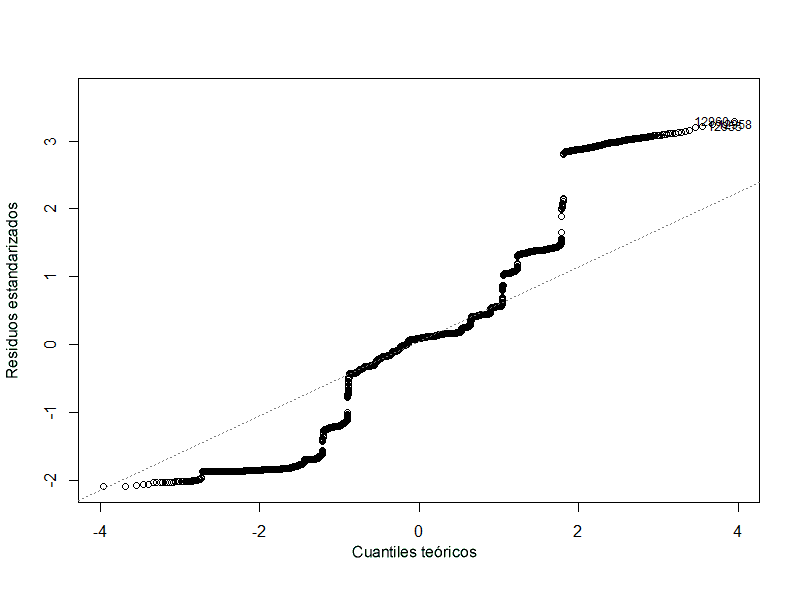
\includegraphics[width=.75\textwidth]{images/t/qq-t.png}
    }
    \subfigure[Residuos contra Valores Ajustados]{
        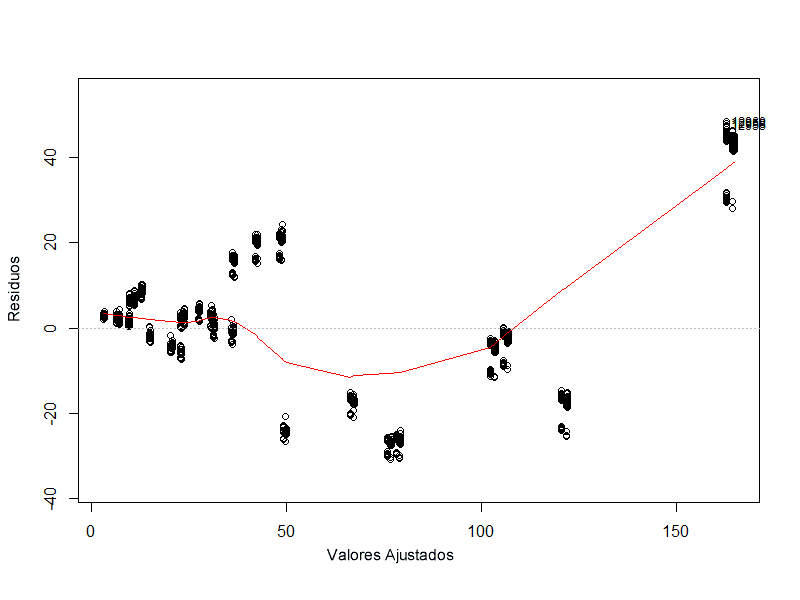
\includegraphics[width=.75\textwidth]{images/t/rvf-t.png}
    }
    \caption{Exploración visual de la normalidad y homogeneidad de varianza en los datos de tiempo sin transformaciones.}
    \label{fig:sin-transformacion}
\end{figure}


\begin{figure}[H]
    \centering
        \small{
        \begin{alltt}
        
        
            > lillie.test(data-t)
                Lilliefors (Kolmogorov-Smirnov) normality test
            data:  data-t
            D = 0.2085, p-value < 2.2e-16
        \end{alltt}
        }
    
    \caption{Prueba de Lilliefors para normalidad en R. El estadístico es mayor que el valor-p por lo que los datos no son normales.}
    \label{fig:lillie-t}
\end{figure}

\begin{figure}[H]
    \centering
        \small{
        \begin{alltt}
        
        
            > levene.test(data-t, data-grupo)
                modified robust Brown-Forsythe Levene-type test 
                based on the absolute deviations from the median
            data:  data-t
            Test Statistic = 21.8013, p-value < 2.2e-16
        \end{alltt}
        }
    \caption{Prueba de Levene para homogeneidad de varianzas en R. El estadístico es mayor que el valor-p por lo que los datos no tiene varianzas homogéneas.}
    \label{fig:levene-t}
\end{figure}




Según \cite{Montgomery2001} en el caso de que los supuestos de ANOVA no se cumplan se pueden tomar varios caminos:
\begin{enumerate}
    \item Aplicar transformaciones a los datos para que cumplan los supuestos y hacer un análisis basado en los nuevos datos.
    \item Utilizar un Modelo Lineal Generalizado.
    \item Usar el método Box-Cox.
    
\end{enumerate}

Todas las estrategias se siguieron y fallaron. A continuación, se presentara el detalle de cada una y la solución final, que consistía en hacer una transformación por rangos\cite{SAS2004}.

%Todas las estrategias se siguieron y fallaron. A continuación, se presentara el detalle de cada una y la solución final, que fue consultada con una experta en estadística de la Unidad de Servicios en Estadística\footnote{\url{http://www.estadistica.ucr.ac.cr/contenido/uses/}} (USES) de la Escuela de Estadística de la Universidad de Costa Rica y que consistía en hacer una transformación por rangos, o que hace que los supuestos de ANOVA se puedan descartar\cite{SAS2004}.

\subsubsection{Transformaciones}

Según la literatura, se pueden aplicar transformaciones según se vea conveniente. Para este caso, se aplicaron las transformaciones de potencia $e$, raíz cuadrada y logaritmo base 10. Estas son las más comunes y a su vez las que tienen más sentido a la hora de la interpretación de los nuevos datos transformados: una transformación de potencia o logaritmo amplía o reduce la distancia de los puntos más altos, en este caso, los tiempos de mayor duración. Es mucho más complejo interpretar una transformación como la siguiente:
\begin{equation}
t-transformado = (t + 24)^2 - sen(2*\pi * t)
\end{equation}

Desgraciadamente ninguna de éstas transformaciones normalizó o cumplió la homogeneidad de varianzas, la exploración visual se hizo como al inicio y reveló los \textbf{mismos problemas}. Las figuras \ref{fig:transformacion-e}, \ref{fig:transformacion-log} y \ref{fig:transformacion-sqrt} muestran los gráficos Q-Q y RvVA de estas transformaciones. En todos los gráficos Q-Q se nota como los puntos se alejan de la línea de tendencia. Los gráficos RvAF también tiene patrones bien marcados, de conos o cúmulos de puntos.



\begin{figure}[H]
\centering
    \subfigure[Cuantiles contra Cuantiles de la Transformación con potencia $e$.]{
        \centering
        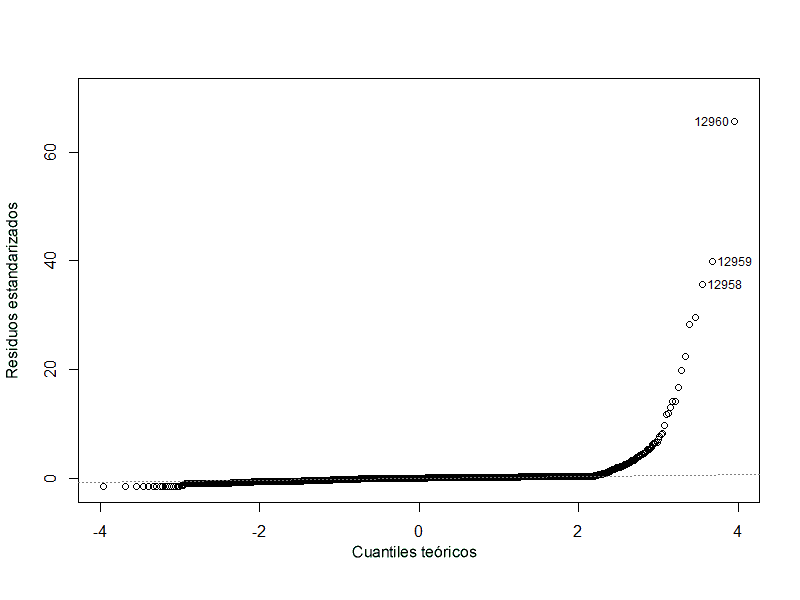
\includegraphics[width=0.75\textwidth]{images/t/qq-e.png}
    }
    \subfigure[Residuos contra Valores Ajustados de la Transformación con potencia $e$.]{
        \centering
        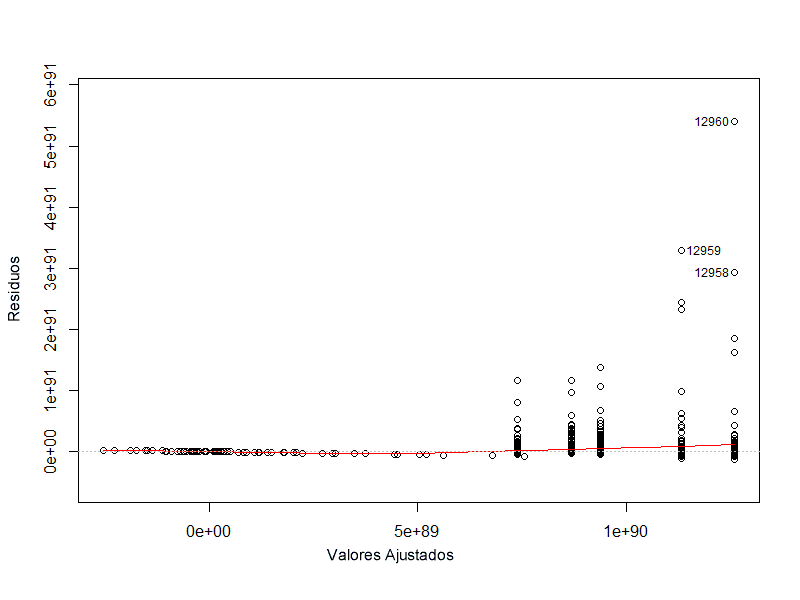
\includegraphics[width=0.75\textwidth]{images/t/rvf-e.png}
    }
\caption{Exploración visual de la normalidad y homogeneidad de varianza en los datos de tiempo transformados con una potencia $e$.}
\label{fig:transformacion-e}
\end{figure}


\begin{figure}[H]
\centering
    \subfigure[Cuantiles contra Cuantiles de la Transformación con logaritmo base 10.]{
        \centering
        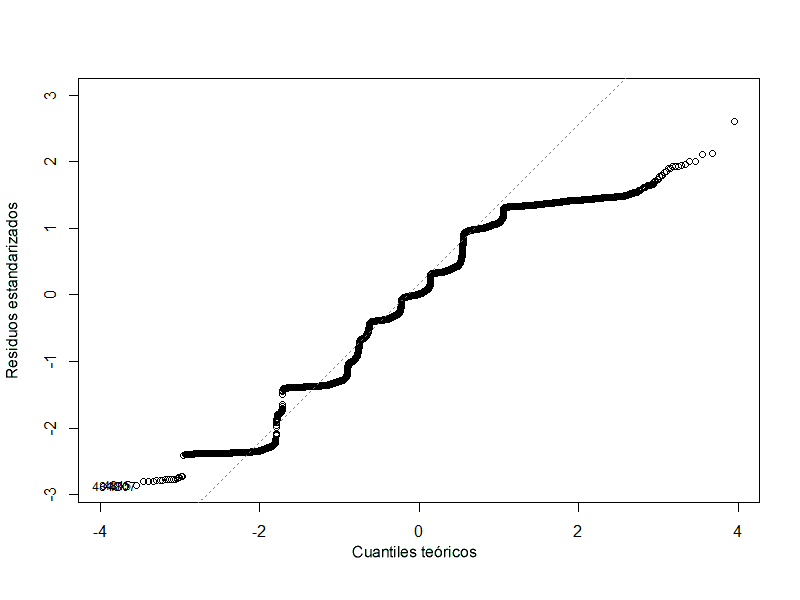
\includegraphics[width=0.75\textwidth]{images/t/qq-log.png}
    }
    \subfigure[Residuos contra Valores Ajustados de la Transformación con logaritmo base 10.]{
        \centering
        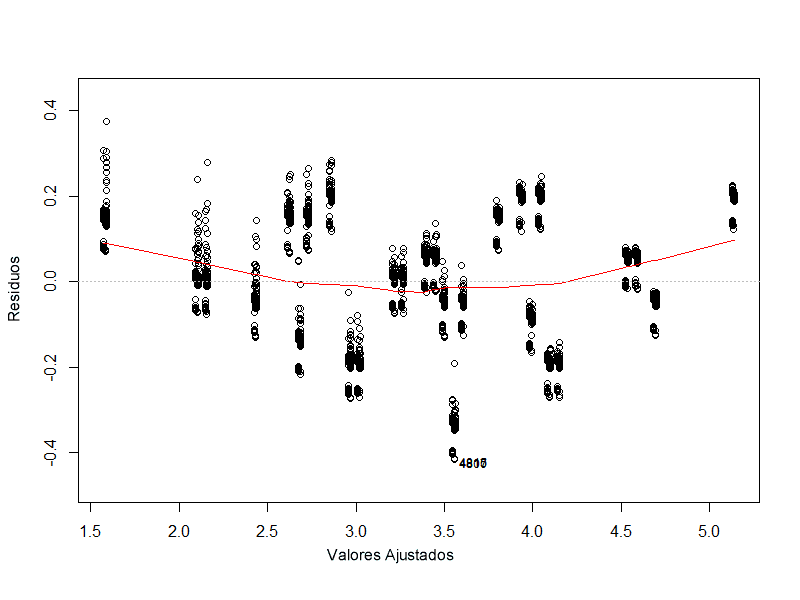
\includegraphics[width=0.75\textwidth]{images/t/rvf-log.png}
    }
\caption{Exploración visual de la normalidad y homogeneidad de varianza en los datos de tiempo transformados con una logaritmo base 10.}
\label{fig:transformacion-log}
\end{figure}


\begin{figure}[H]
\centering
    \subfigure[Cuantiles contra Cuantiles de la Transformación con raíz cuadrada.]{
        \centering
        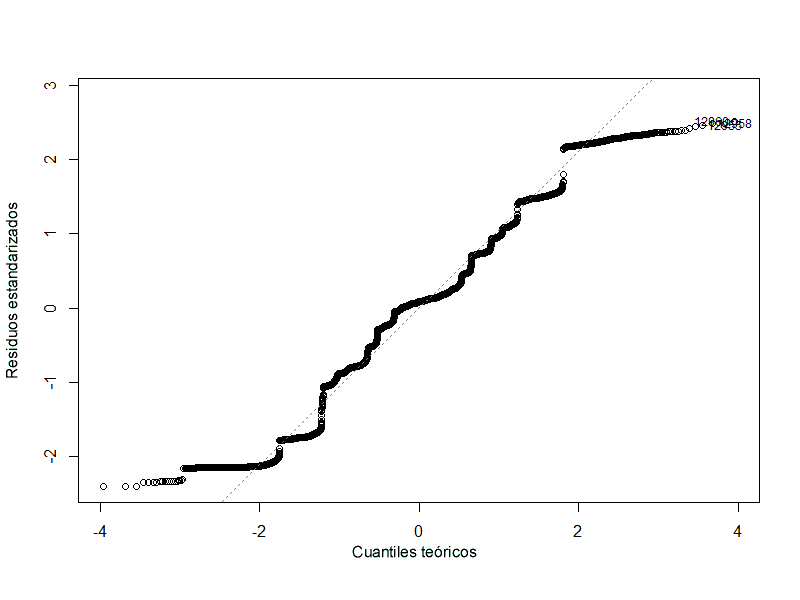
\includegraphics[width=0.75\textwidth]{images/t/qq-sqrt.png}
    }
    \subfigure[Residuos contra Valores Ajustados de la Transformación con raíz cuadrada.]{
        \centering
        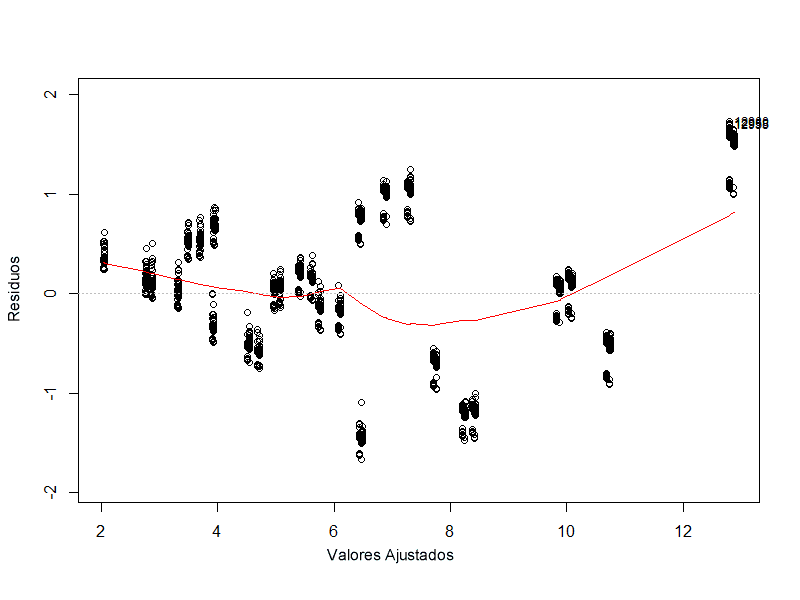
\includegraphics[width=0.75\textwidth]{images/t/rvf-sqrt.png}
    }
\caption{Exploración visual de la normalidad y homogeneidad de varianza en los datos de tiempo transformados con una raíz cuadrada.}
\label{fig:transformacion-sqrt}
\end{figure}

\subsubsection{Modelo Lineal Generalizado}

El Modelo Lineal Generalizado (GLM por sus siglas en inglés) es una generalización de la regresión lineal, que no toma como un hecho la distribución gaussiana del error en la variable de respuesta\cite{Montgomery2001}.

Para utilizar un GLM se necesita:
\begin{itemize}
    \item Una función de enlace.
    \item Una distribución de probabilidad para los errores.
\end{itemize}

La escogencia de estos dos requerimientos hace que nuevamente se hagan supuestos sobre los datos y debido a esto, se descartó.


\subsubsection{Método Box-Cox}

El método Box-Cox\cite{Sakia1992} es una función de optimización, donde se minimiza la desviación estándar de un conjunto de datos al calcular una transformación de potencia $\lambda$.
La figura \ref{fig:box-cox} muestra el resultado del proceso Box-Cox en R, donde se puede notar que la transformación óptima es cerca de $-1$.


\begin{figure}[H]
    \centering
    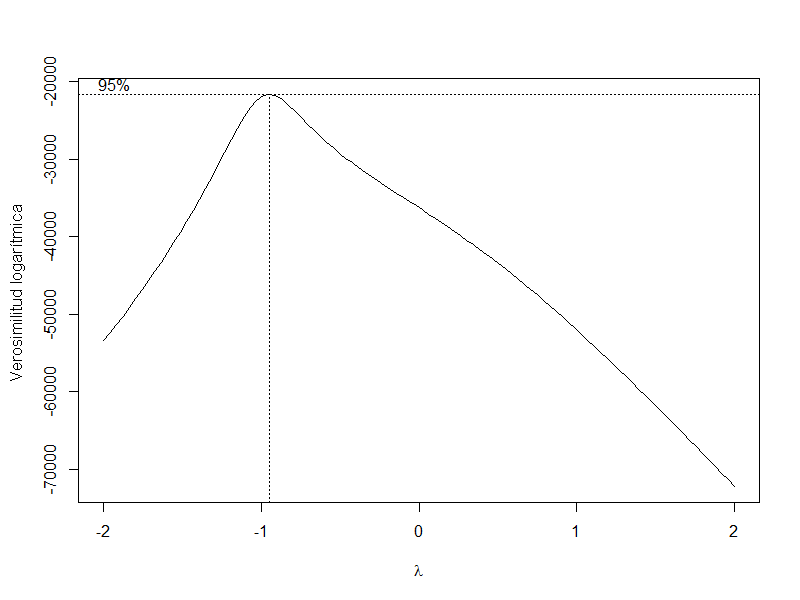
\includegraphics[width=0.75\textwidth]{images/t/box-cox.png}
    \caption{Método Box-Cox. El punto óptimo $\lambda$, con un 95\% de confianza se encuentra cerca de -1.}
    \label{fig:box-cox}
\end{figure}


Al aplicar una transformación de potencia $-1$, la exploración visual nuevamente falla al validar los supuestos de ANOVA. La figura \ref{fig:transformacion-bc} muestra el gráfico Q-Q y RvAF de la transformación sugerida por el método Box-Cox.

\begin{figure}[H]
\centering
    \subfigure[Cuantiles contra Cuantiles de la Transformación con el método Box-Cox.]{
        \centering
        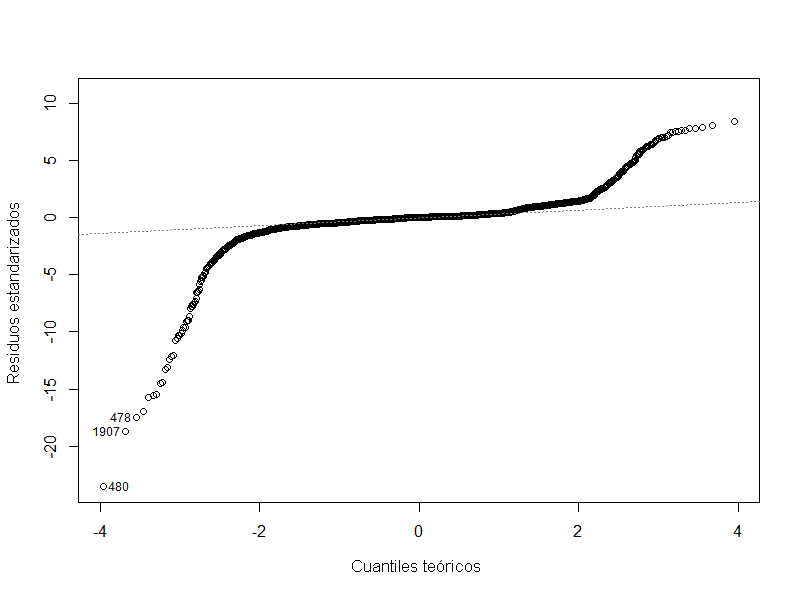
\includegraphics[width=0.75\textwidth]{images/t/qq-bc.png}
    }
    \subfigure[Residuos contra Valores Ajustados de la Transformación con el método Box-Cox.]{
        \centering
        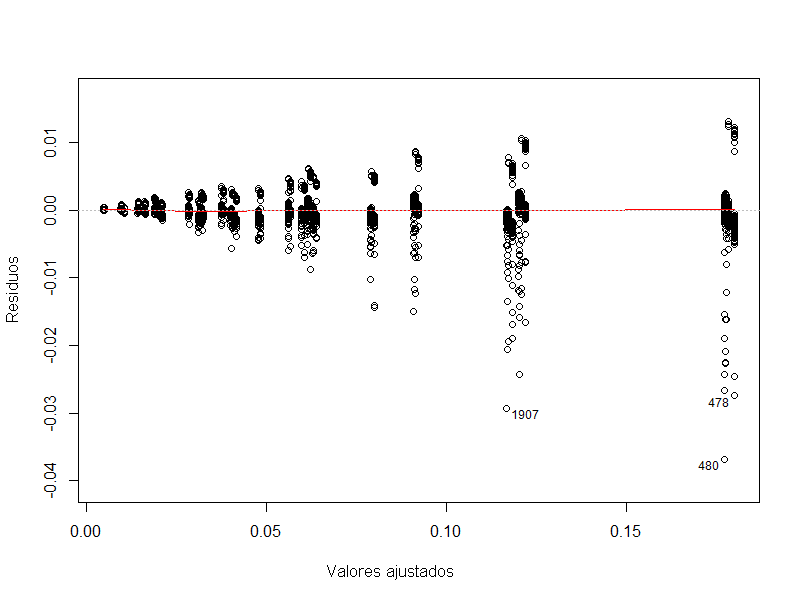
\includegraphics[width=0.75\textwidth]{images/t/rvf-bc.png}
    }
\caption{Exploración visual de la normalidad y homogeneidad de varianza en los datos de tiempo transformados con el método Box-Cox.}
\label{fig:transformacion-bc}
\end{figure}


\subsubsection{Transformación por Rangos}

Luego de haber agotado las opciones brindadas por la literatura, se decidió consultar a la USES, donde se concertaron dos reuniones de trabajo donde se decidió por criterio experto hacer una transformación por Rangos, que elimina los supuestos de ANOVA\cite{USES2014}\cite{SAS2004}.

La transformación por rangos es un proceso estadístico que toma el mejor valor de una variable y le asigna el rango de 1, toma el siguiente mejor valor y asigna el rango de 2 sucesivamente hasta el peor valor de la variable y se le asigna el ultimo rango. 

Para los tiempos en la TT, un tiempo bajo es un buen valor y un tiempo alto es un valor malo, así, el tiempo de 5,177 segundos tiene el rango 1 y el tiempo de 216,606 segundos, el rango 12960. Esta conversión sigue la función en la gráfica de la figura \ref{fig:rank-t}.

\begin{figure}[H]
    \centering
    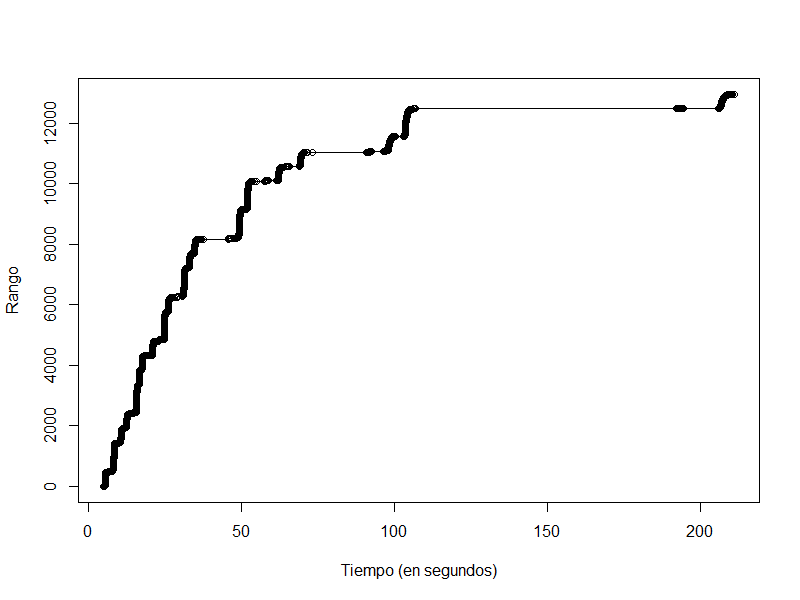
\includegraphics[width=0.75\textwidth]{images/t/rank.png}
    \caption{Transformación por rangos de los datos de tiempo tomados en el experimento A.}
    \label{fig:rank-t}
\end{figure}

\subsection{Análisis de resultados}

Una vez superado los supuestos de ANOVA, se procedió a hacer el análisis de los tiempos transformados a rangos.

El procedimiento \texttt{aov} en R es el utilizado para hacer el análisis de varianza. Esta función reporta dos salidas: una tabla de ANOVA y el cuadro resumen, de los cuales la tabla es la que nos interesa.

La figura \ref{fig:anova-t} muestra la invocación de la función \texttt{aov} y la tabla \ref{tab:anovaA} muestra la relevancia de cada combinación de factores.

\begin{figure}[H]
    \centering
            \small
            \begin{alltt}
            
            
            > aov(rank(t) ~ dTau * dRho * dPhi * cobertura)
            \end{alltt}
    \caption{Invocación de la función aov para Análisis de Varianza en R. El parámetro recibido muestra las relaciones entre las variables: $rank(t)$ la variable de respuesta se debe analizar en función de $\Delta \tau$, $\Delta \rho$, $\Delta \phi$, tipo de cobertura y todas sus combinaciones.}
    \label{fig:anova-t}
\end{figure}


\begin{table}\renewcommand{\tabcolsep}{3pt}
    \centering
    \small
    \begin{tabular}{lrrrrrr}
        \hline 
        Factor & Df & Sum Sq & Mean Sq & F-value & Pr($>$F) & Sig.\\
        \hline 
        \textbf{dTau} & 1 & 6.056e+10 & 6.056e+10 & 9.681e+04 & $<$2e-16 & 0\\
        \textbf{dPhi} & 1 & 7.188e+10 & 7.188e+10 & 1.149e+05 & $<$2e-16 & 0\\
        \textbf{dRho} & 1 & 3.796e+10 & 3.796e+10 & 6.068e+04 & $<$2e-16 & 0\\
        \textbf{cobertura} & 4 & 2.135e+07 & 5.338e+06 & 8.533e+00 & 7.15e-07 & 0\\
        \textbf{dTau:dPhi} & 1 & 5.291e+07 & 5.291e+07 & 8.458e+01 & $<$2e-16 & 0\\
        \textbf{dTau:dRho} & 1 & 1.383e+08 & 1.383e+08 & 2.211e+02 & $<$2e-16 & 0\\
        dPhi:dRho & 1 & 1.108e+03 & 1.108e+03 & 2.000e-03 & 0.966 & \\
        dTau:cobertura & 4 & 2.380e+06 & 5.951e+05 & 9.510e-01 & 0.433 & \\
        dPhi:cobertura & 4 & 8.064e+04 & 2.016e+04 & 3.200e-02 & 0.998 & \\
        dRho:cobertura & 4 & 1.340e+05 & 3.351e+04 & 5.400e-02 & 0.995 & \\
        \textbf{dTau:dPhi:dRho} & 1 & 2.709e+09 & 2.709e+09 & 4.330e+03 & $<$2e-16 & 0\\
        dTau:dPhi:cobertura & 4 & 1.172e+06 & 2.929e+05 & 4.680e-01 & 0.759 & \\
        dTau:dRho:cobertura & 4 & 6.292e+04 & 1.573e+04 & 2.500e-02 & 0.999 & \\
        dPhi:dRho:cobertura & 4 & 8.207e+05 & 2.052e+05 & 3.280e-01 & 0.859 & \\
        dTau:dPhi:dRho:cobertura & 4 & 4.000e+05 & 1.000e+05 & 1.600e-01 & 0.959 &\\
        Residuos & 12920 & 8.082e+09 & 6.256e+05\\
        \hline
    \end{tabular}
    \caption{Tabla ANOVA para los rangos de tiempo del experimento A.}
    \label{tab:anovaA}
\end{table}

La tabla indica que existen siete combinaciones de factores que influyen sobre la variable de respuesta. Estos son los cuatro factores principales, las interacción de segundo nivel $\Delta \tau$ con $\Delta \rho$ y $\Delta \tau$ con $\Delta \phi$, y la interacción de tercer nivel de los parámetros de frecuencia.

El efecto de los factores principales se evidencia en la figura \ref{tab:ME-A}. Todos los parámetros de frecuencia muestran un decremento en tiempo mientras más crecen (un rango alto representa un tiempo largo), lo que es esperable: \textbf{a más fino el barrido, más tiempo se tarda extraer las características}. 

\begin{figure}[H]
    \centering
    \subfigure[$\Delta \tau$]{
    	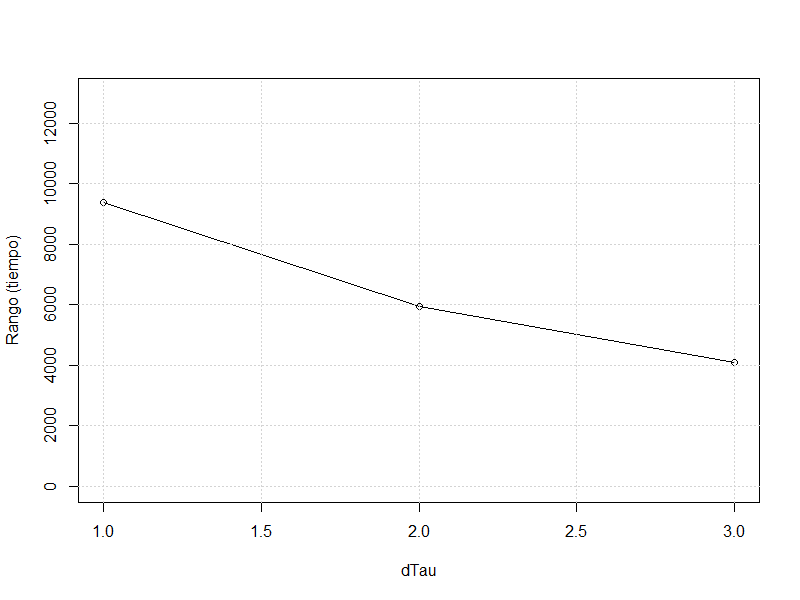
\includegraphics[width=0.4\textwidth]{images/t/t-MEdTau.png}
    }
    \subfigure[$\Delta \rho$]{
         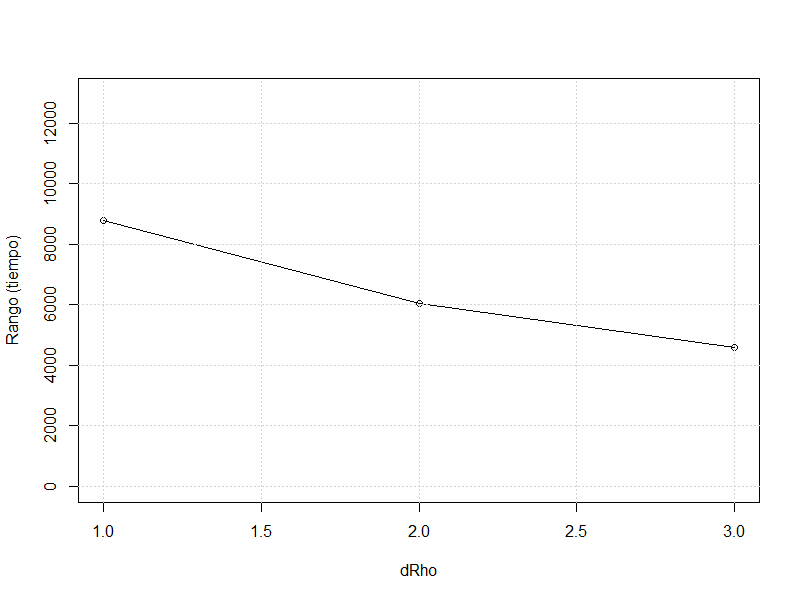
\includegraphics[width=0.4\textwidth]{images/t/t-MEdRho.png}
    }
    \subfigure[$\Delta \phi$]{
        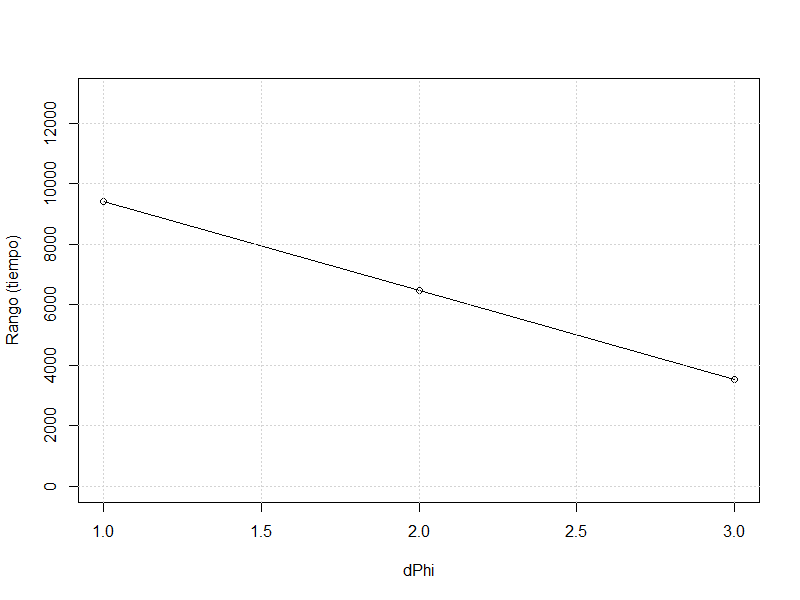
\includegraphics[width=0.4\textwidth]{images/t/t-MEdPhi.png}
    }
    \subfigure[Tipo de cobertura de terreno]{
        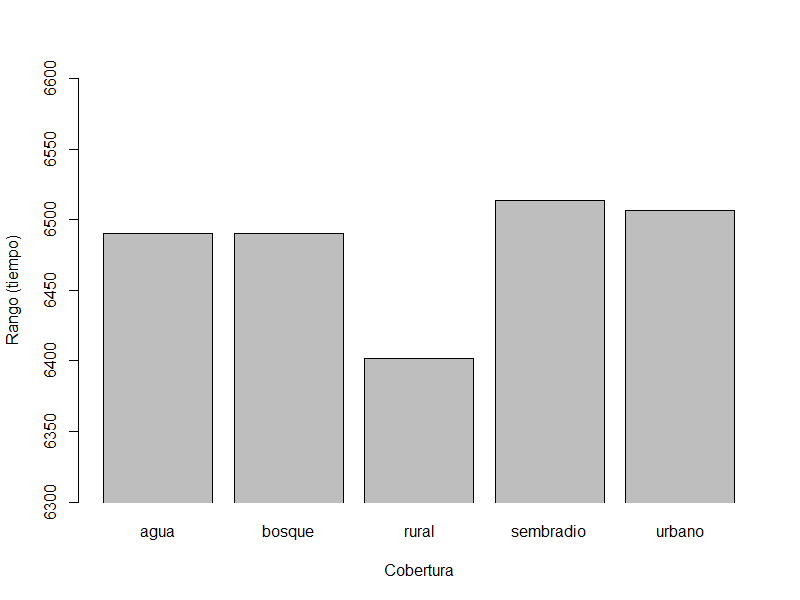
\includegraphics[width=0.4\textwidth]{images/t/t-MEcobertura.png}
    }
\caption{Promedio del efecto de los factores principales del experimento A.}
\label{tab:ME-A}
\end{figure}

El efecto que tiene el tipo de cobertura sobre el tiempo es poco, pero dado el análisis, es significativo. El tipo de cobertura rural, aunque muestre un mejor tiempo en promedio, la diferencia es ínfima: del rango 6400 al 6500 la diferencia es de 0,03033333 segundos.

Las interacciones de segundo nivel se muestran en la figura \ref{tab:2I-A}. La subfigura (a) expone el promedio de los rangos cuando $\Delta \tau$ y $\Delta \phi$ cambian juntos, de igual manera pero con $\Delta \rho$ en la subfigura (b). 

\begin{figure}[H]

    \centering
    \subfigure[$\Delta \tau$ y $\Delta \phi$]{
    	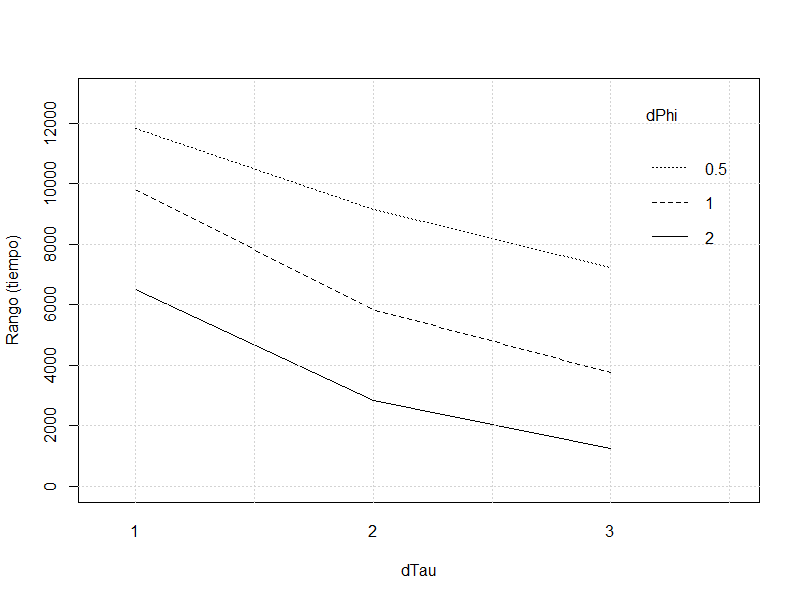
\includegraphics[width=0.75\textwidth]{images/t/t-2IdTau-dPhi.png}
    }
    \subfigure[$\Delta \tau$ y $\Delta \rho$]{
        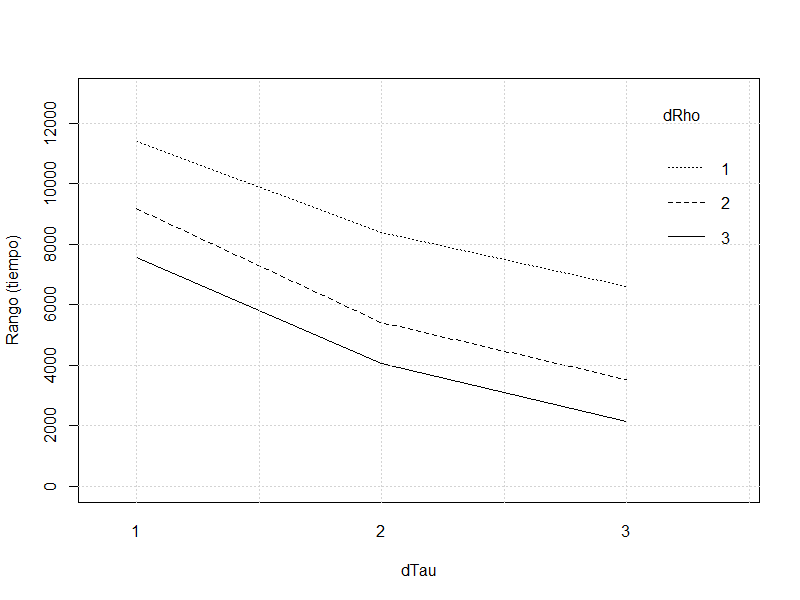
\includegraphics[width=0.75\textwidth]{images/t/t-2IdTau-dRho.png}
    }
\caption{Promedio de interacciones de segundo nivel en el experimento A.}
\label{tab:2I-A}
\end{figure}

En ambos, se muestra un comportamiento decreciente en los rangos y tiempos a como se incrementan los parámetros de frecuencia, siendo los puntos extremos nuevamente las combinaciones $\Delta \tau=3$, $\Delta \phi=2$ y $\Delta \tau=3$, $\Delta \rho=3$. El efecto es ligeramente más marcado con $\Delta \phi$, donde los rangos son más bajos.

Por último, la interacción de tercer nivel se muestra en la figura \ref{tab:3I-A}. Esta interacción toma en cuenta todas las variaciones de los parámetros de frecuencia y deja por fuera el tipo de cobertura de terreno.

En todos los casos el comportamiento no es una sorpresa,  es decreciente en bloques: con $\Delta \tau=1$ se tarda más en promedio, con cualquier valor de $\Delta \rho$ y $\Delta \phi$, que con $\Delta \tau=3$. Esto significa, que al igual que como se indican con las interacciones anteriores, el tiempo de extracción decrece a como los parámetros aumentan ya sea de manera independiente o conjunta.



\begin{figure}[H]
    \centering
    \subfigure[$\Delta \tau$=1 y $\Delta \rho$ y $\Delta \phi$]{
    	
		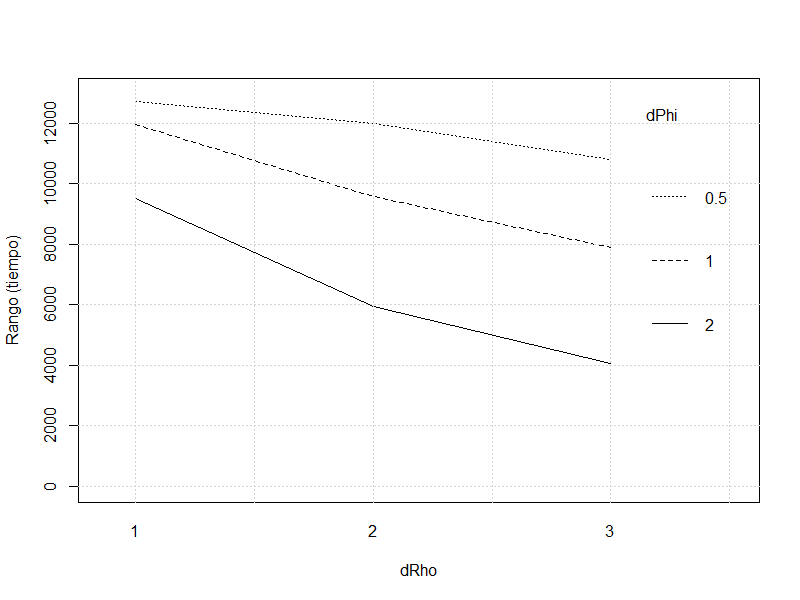
\includegraphics[width=0.5\textwidth]{images/t/t-3I-t1.png}
    }
    \subfigure[$\Delta \tau$=2 y $\Delta \rho$ y $\Delta \phi$]{
        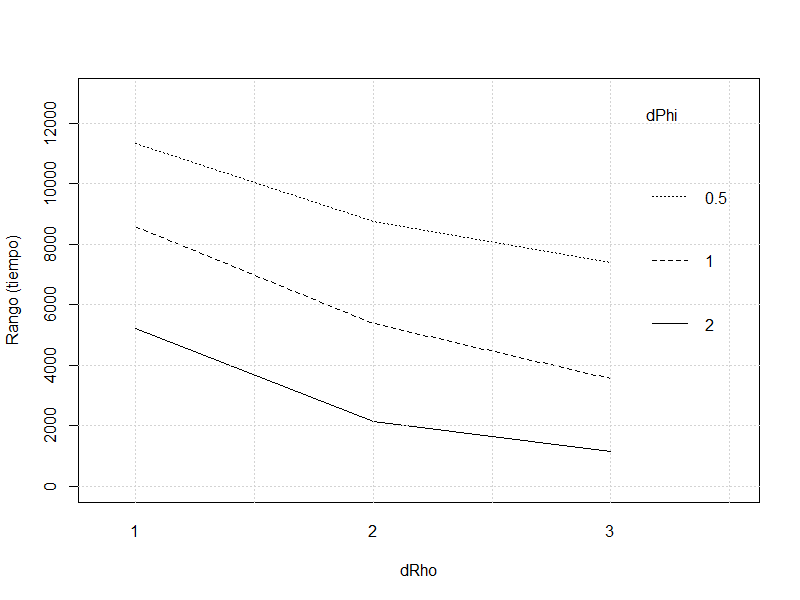
\includegraphics[width=0.5\textwidth]{images/t/t-3I-t2.png}
    }
    \subfigure[$\Delta \tau$=3 y $\Delta \rho$ y $\Delta \phi$]{
        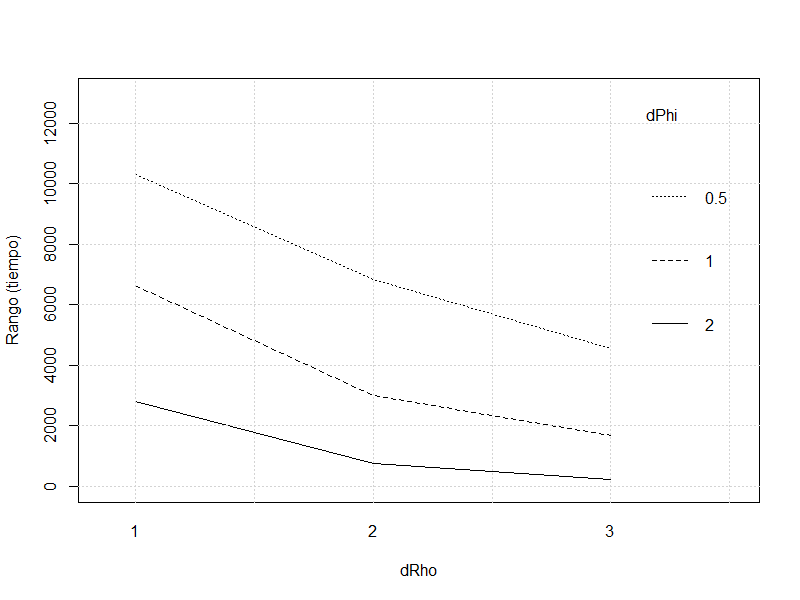
\includegraphics[width=0.5\textwidth]{images/t/t-3I-t3.png}
    }
\caption{Promedio de la interacción de tercer nivel para el experimento A.}
\label{tab:3I-A}
\end{figure}


%%%%%%%%%%%%%%%%%%%%%%%%%%%%%%%%%%%%%%%%%%%%%%%%%%%%%%%%%%%%%%%%%%%%%%%
%%%%%%%%%%%%%%%%%%%%%%%%%%%%%%%%%%%%%%%%%%%%%%%%%%%%%%%%%%%%%%%%%%%%%%%
%%%%%%%%%%%%%%%%%%%%%%%%%%%%%%%%%%%%%%%%%%%%%%%%%%%%%%%%%%%%%%%%%%%%%%%
%%%%%%%%%%%%%%%%%%%%%%%%%%%%%%%%%%%%%%%%%%%%%%%%%%%%%%%%%%%%%%%%%%%%%%%
%%%%%%%%%%%%%%%%%%%%%%%%%%%%%%%%%%%%%%%%%%%%%%%%%%%%%%%%%%%%%%%%%%%%%%%

\section{Experimento B}

\subsection{Verificación de supuestos}

Al igual que con el experimento A, se realizó una exploración visual que rechazó los supuestos de ANOVA, como se indica en la figura \ref{fig:sin-transformacion-p}. También se confirmó con la prueba de Lilliefors como lo demuestra la figura \ref{fig:lillie-p}; el estadístico calculado descarta normalidad, por lo que se prosiguió a aplicar transformaciones a los datos.

\begin{figure}[H]
    \centering
        \small{
        \begin{alltt}
        
        
            > lillie.test(data-p)
                Lilliefors (Kolmogorov-Smirnov) normality test
            data:  data-p
            D = 0.3546, p-value < 2.2e-16
        \end{alltt}
        }
    \caption{Prueba de Lilliefors para normalidad en R. El estadístico es mayor que el valor-p por lo que los datos no son normales.}
    \label{fig:lillie-p}
\end{figure}

\begin{figure}[H]
    \centering
    \subfigure[Cuantiles contra Cuantiles.]{
        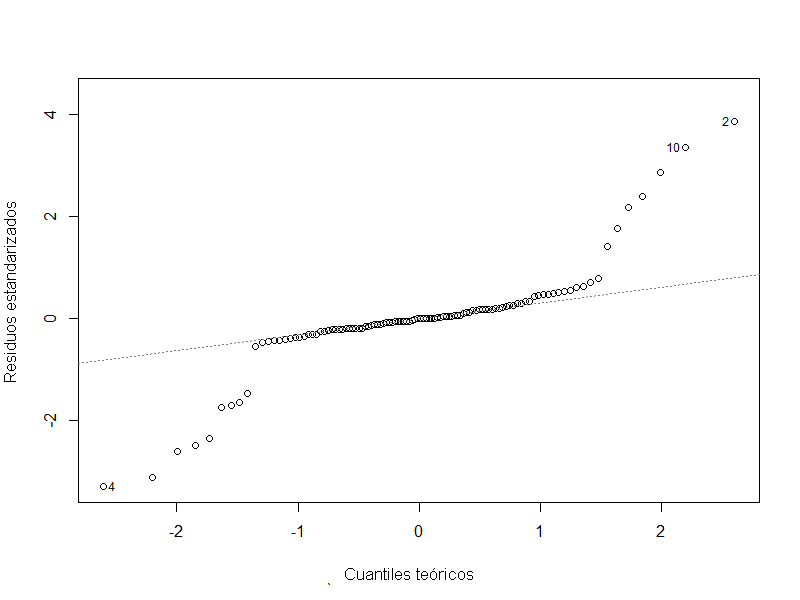
\includegraphics[width=.75\textwidth]{images/p/qq-p.png}
    }
    \subfigure[Residuos contra Valores Ajustados.]{
        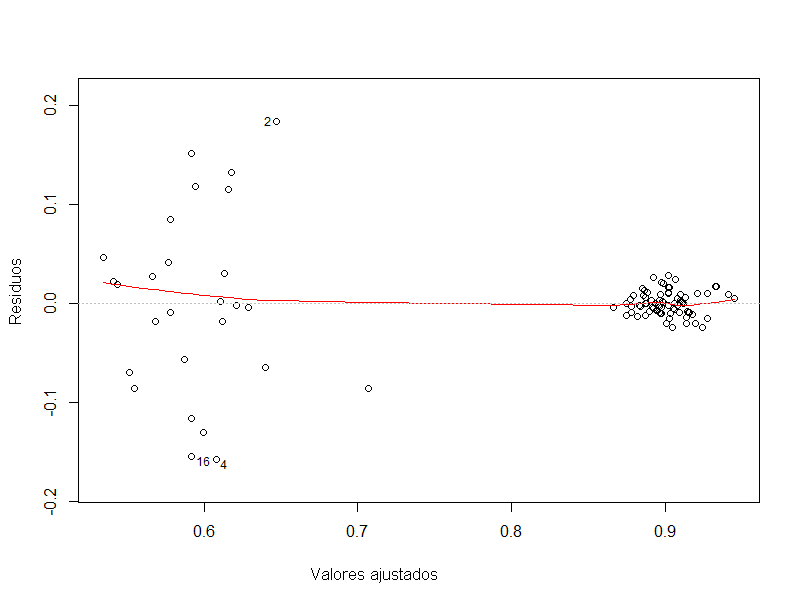
\includegraphics[width=.75\textwidth]{images/p/rvf-p.png}
    }
    \caption{Exploración visual de la normalidad y homogeneidad de varianza en los datos de precisión.}
    \label{fig:sin-transformacion-p}
\end{figure}

\subsubsection{Transformaciones}

Las transformaciones aplicadas a los datos de tiempo fueron aplicadas a los datos de precisión: potencia $e$, raíz cuadrada y logaritmo base 10.

En todos los casos, los supuestos fueron rechazados. Para cada transformación, potencia $e$, raíz cuadrada y logaritmo base 10, se muestran los gráficos Q-Q y RvAF, respectivamente en las figuras \ref{fig:transformacion-e-p} \ref{fig:transformacion-log-p} \ref{fig:transformacion-sqrt-p}.


\begin{figure}[H]
\centering
    \subfigure[Cuantiles contra Cuantiles de la Transformación con potencia $e$.]{
        \centering
        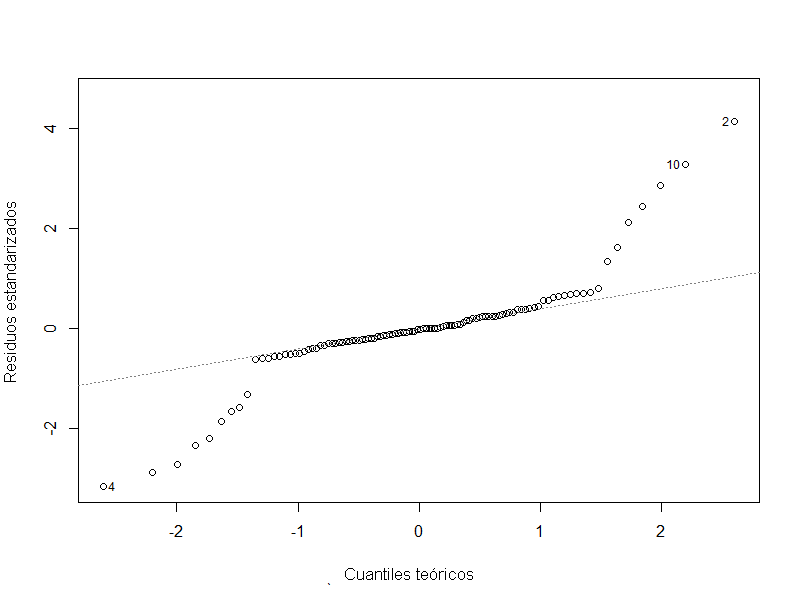
\includegraphics[width=0.75\textwidth]{images/p/qq-e.png}
    }
    \subfigure[Residuos contra Valores Ajustados de la Transformación con potencia $e$.]{
        \centering
        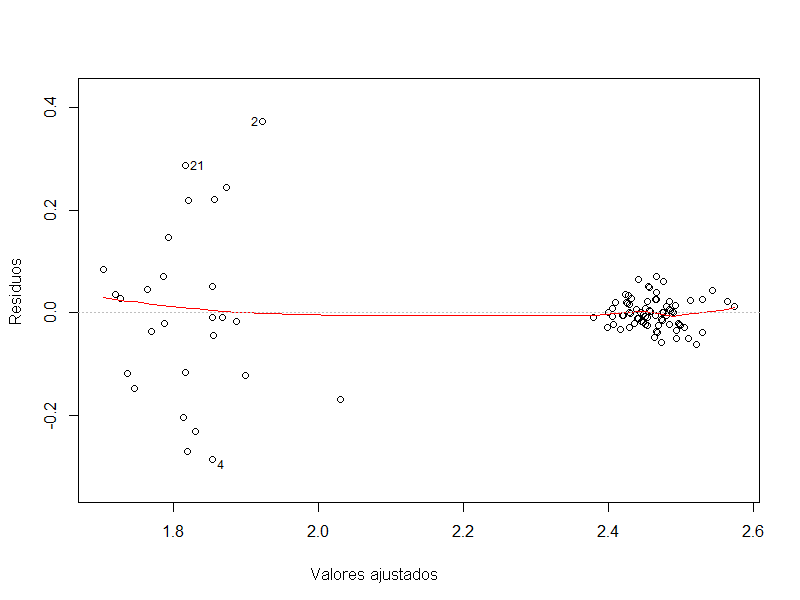
\includegraphics[width=0.75\textwidth]{images/p/rvf-e.png}
    }
\caption{Exploración visual de la normalidad y homogeneidad de varianza en los datos de precisión transformados con una potencia $e$.}
\label{fig:transformacion-e-p}
\end{figure}


\begin{figure}[H]
\centering
    \subfigure[Cuantiles contra Cuantiles de la Transformación con logaritmo base 10.]{
        \centering
        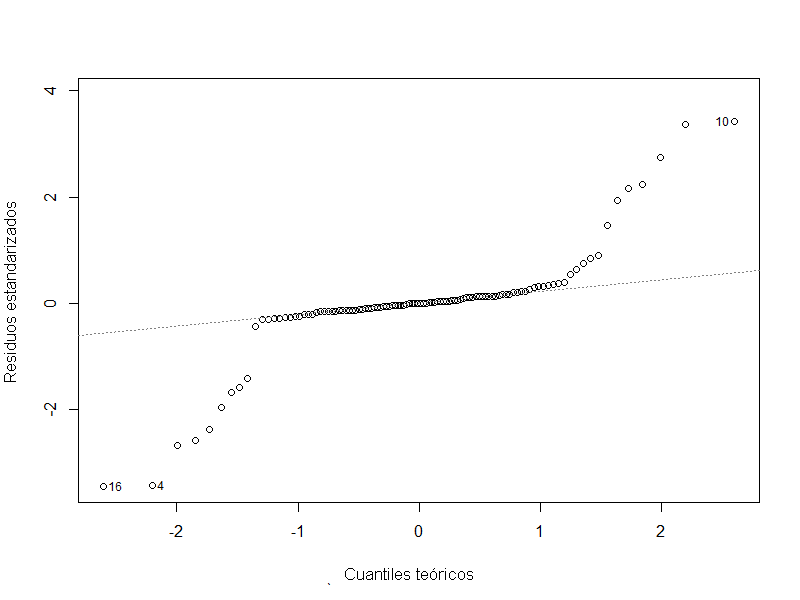
\includegraphics[width=0.75\textwidth]{images/p/qq-log.png}
    }
    \subfigure[Residuos contra Valores Ajustados de la Transformación con logaritmo base 10.]{
        \centering
        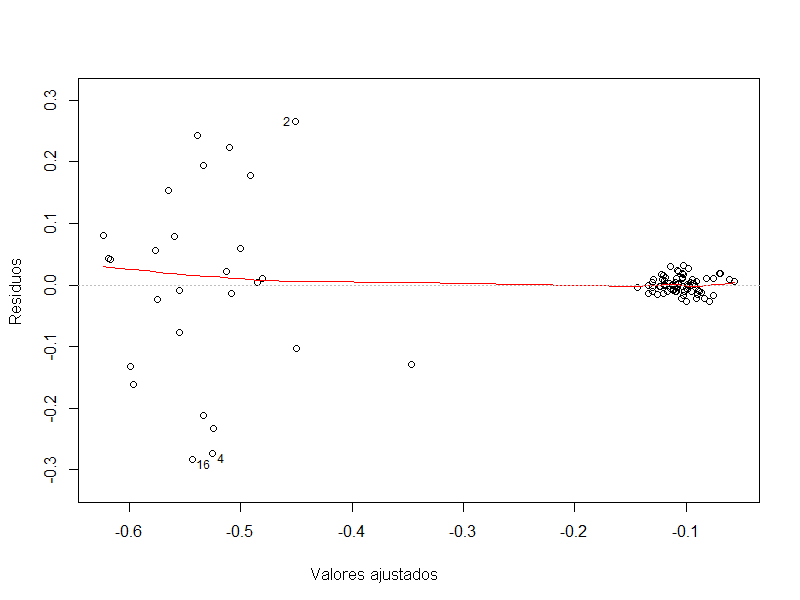
\includegraphics[width=0.75\textwidth]{images/p/rvf-log.png}
    }
\caption{Exploración visual de la normalidad y homogeneidad de varianza en los datos de precisión transformados con una logaritmo base 10.}
\label{fig:transformacion-log-p}
\end{figure}


\begin{figure}[H]
\centering
    \subfigure[Cuantiles contra Cuantiles de la Transformación con raíz cuadrada.]{
        \centering
        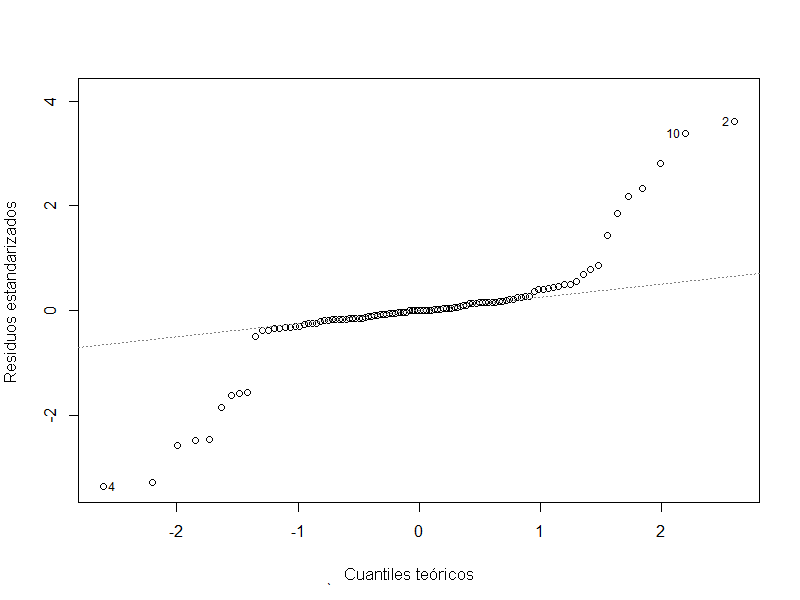
\includegraphics[width=0.75\textwidth]{images/p/qq-sqrt.png}
    }
    \subfigure[Residuos contra Valores Ajustados de la Transformación con raíz cuadrada.]{
        \centering
        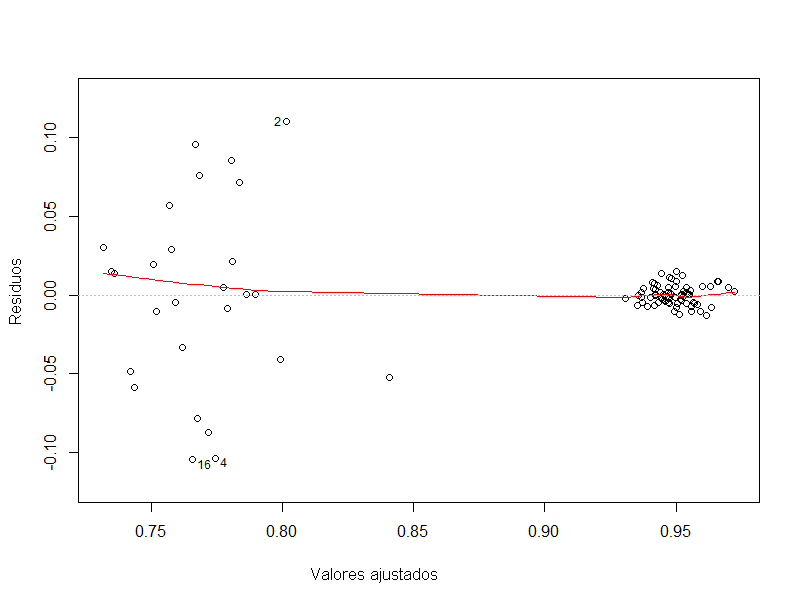
\includegraphics[width=0.75\textwidth]{images/p/rvf-sqrt.png}
    }
\caption{Exploración visual de la normalidad y homogeneidad de varianza en los datos de precisión transformados con una raíz cuadrada.}
\label{fig:transformacion-sqrt-p}
\end{figure}


\subsubsection{Modelo Lineal Generalizado}

El GLM fue descartado dadas las mismas razones que se plantean en el experimento A: no se pueden afirmar supuestos sobre distribución de errores de los datos de precisión ni establecer una función de enlace sin que sea de forma arbitraria.

Al igual que en el experimento A, se procedió a aplicar el método Box-Cox con la expectativa de que dicha transformación confirme los supuestos.

\subsubsection{Método Box-Cox}

El método Box-Cox reporta un valor $\lambda$ óptimo cerca de 2, como lo muestra la figura \ref{fig:box-cox-p}, por lo que se aplicó una transformación de potencia $2$ a los datos.

Infortunadamente la transformación rechaza los supuestos nuevamente. La figura \ref{fig:transformacion-bc-p} muestra la exploración visual que descarta normalidad y homogeneidad de varianzas.

\begin{figure}[H]
    \centering
    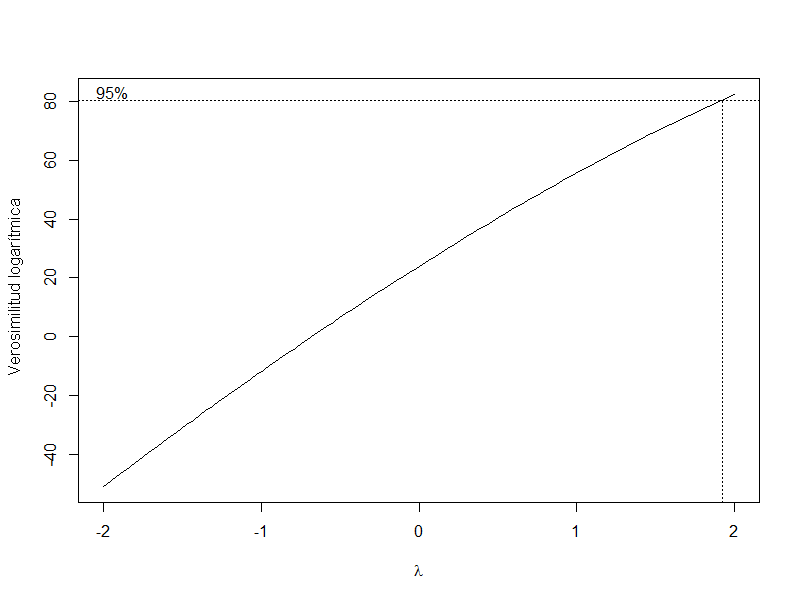
\includegraphics[width=0.75\textwidth]{images/p/box-cox-p.png}
    \caption{Método Box-Cox. El punto óptimo $\lambda$, con un 95\% de confianza se encuentra cerca de 2.}
    \label{fig:box-cox-p}
\end{figure}


\begin{figure}[H]
\centering
    \subfigure[Cuantiles contra Cuantiles de la Transformación con el método Box-Cox.]{
        \centering
        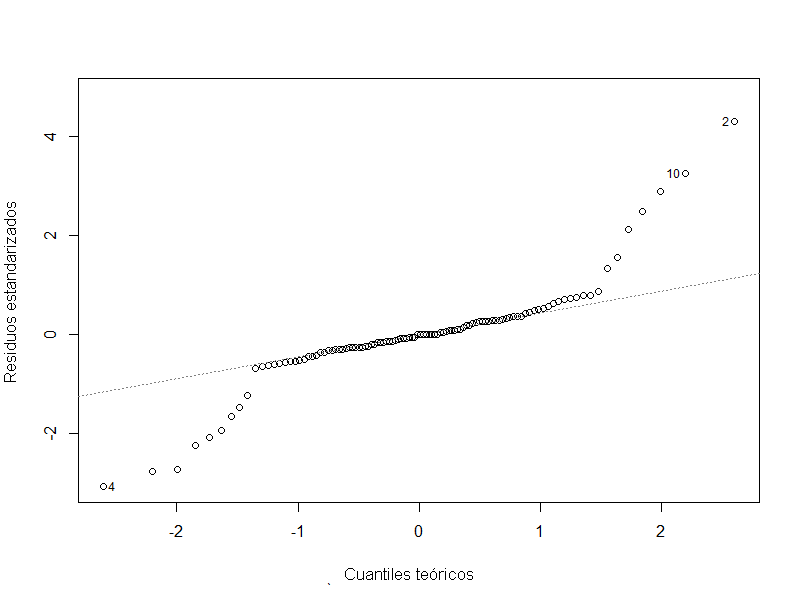
\includegraphics[width=0.75\textwidth]{images/p/qq-bc.png}
    }
    \subfigure[Residuos contra Valores Ajustados de la Transformación con el método Box-Cox.]{
        \centering
        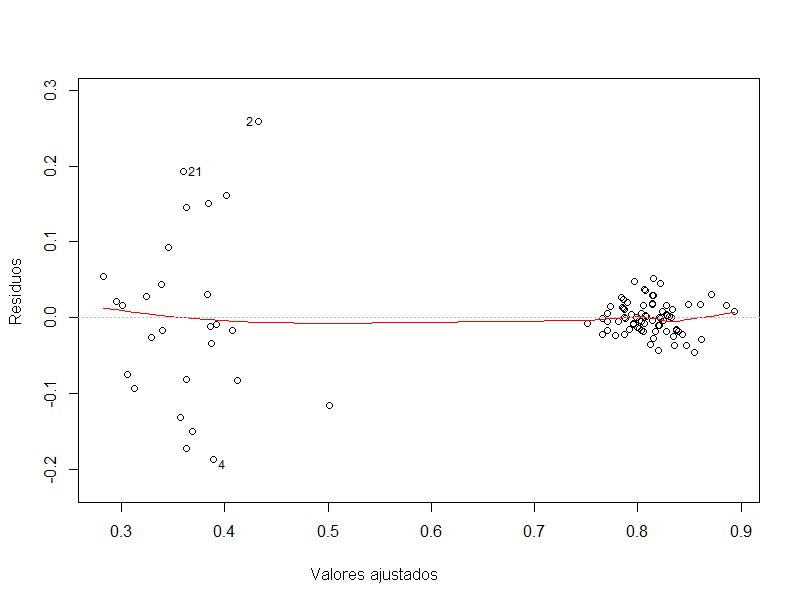
\includegraphics[width=0.75\textwidth]{images/p/rvf-bc.png}
    }
\caption{Exploración visual de la normalidad y homogeneidad de varianza en los datos de precisión transformados con el método Box-Cox.}
\label{fig:transformacion-bc-p}
\end{figure}

Dados estos fallos al verificar los supuestos, se optó por la misma solución que en el experimento A y aplicar una transformación por rangos.


\subsubsection{Transformación por Rangos}

Se aplicó en este caso una transformación por rangos donde un rango bajo significa una mala precisión, y un rango alto, una buena precisión (inverso al caso de los tiempos).

Así la peor precisión de 0,4375 tendrá el rango 1 y la mejor precisión 0,95 tendrá el rango más alto 212,5. Esta transformación se puede ver en la figura \ref{fig:rank-p}.


\begin{figure}[H]
    \centering
    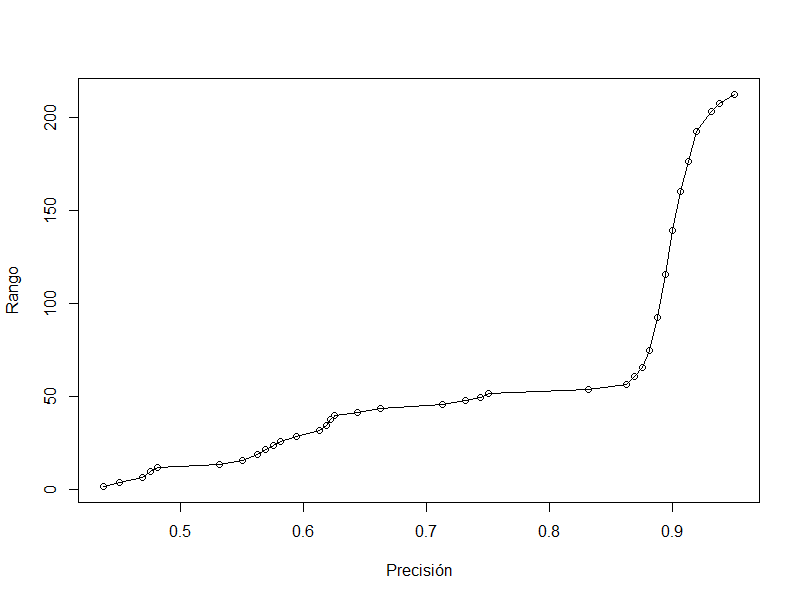
\includegraphics[width=0.75\textwidth]{images/p/rank.png}
    \caption{Transformación por rangos de los datos de precisión tomados en el experimento B.}
    \label{fig:rank-p}
\end{figure}


\subsection{Análisis de Resultados}

La tabla ANOVA se muestra en la figura \ref{tab:anovaB}.
Es preciso recordar que para este experimento, la transformación de los datos hizo que un rango bajo signifique una precisión alta (se puede ver también como el error en la clasificación).



\begin{table}\renewcommand{\tabcolsep}{3pt}
    \centering
    \small
    \begin{tabular}{lrrrrrr}
        \hline 
        Factor & Df & Sum Sq & Mean Sq & F-value & Pr($>$F) & Sig.\\
        \hline 
        \textbf{dTau} & 1 & 1168 & 1168 & 4.622 & 0.034752 & 0.05\\
        dPhi & 1 & 89 & 89 & 0.353 & 0.553947 &\\
        dRho & 1 & 133 & 133 & 0.528 & 0.469773 &\\
        \textbf{clasificador} & 3 & 72454 & 24151 & 95.560 & $<$2e-16 & 0\\
        dTau:dPhi & 1 & 58 & 58 & 0.230 & 0.632989 &\\
        dTau:dRho & 1 & 248 & 248 & 0.979 & 0.325495 &\\
        dPhi:dRho & 1 & 0 & 0 & 0.000 & 0.989759 &\\
        \textbf{dTau:clasificador} & 3 & 5793 & 1931 & 7.641 & 0.000157 & 0\\
        dPhi:clasificador & 3 & 1384 & 461 & 1.825 & 0.149661 &\\
        dRho:clasificador & 3 & 1970 & 657 & 2.598 & 0.058362 & 0.1\\
        dTau:dPhi:dRho & 1 & 462 & 462 & 1.827 & 0.180523 & \\
        dTau:dPhi:clasificador & 3 & 664 & 221 & 0.876 & 0.457247 & \\
        dTau:dRho:clasificador & 3 & 62 & 21 & 0.082 & 0.969620 & \\
        dPhi:dRho:clasificador & 3 & 208 & 69 & 0.275 & 0.843459 & \\
        dTau:dPhi:dRho:clasificador & 3 & 474 & 158 & 0.625 & 0.601146 & \\
        Residuals & 76 & 19208 & 253\\
        \hline
    \end{tabular}
    \caption{Tabla ANOVA para la precisión en la clasificación.}
    \label{tab:anovaB}    
\end{table}


Los factores e interacciones relevantes fueron: $\Delta \tau$, el clasificador y la interacción de segundo nivel entre ellos.

El factor $\Delta \tau$ presenta un efecto tenue sobre la variable de respuesta, sin importar su variación, la precisión se mantiene casi constante. La gráfica en la figura \ref{tab:ME-B} (a) muestra una línea prácticamente horizontal de $\Delta \tau$ contra los rangos de la precisión. 
Por otro lado la subfigura (b) muestra el tipo de clasificador contra los rangos. Aquí las diferencias son muy marcadas entre ellos. 
En promedio LogitBoost y SMO superan a los otros clasificadores, con rangos promedios de 163,64 (precisión de 0,9134259) y 142,90 (precisión de 0,9023148) respectivamente, y Kmeans es el peor de los cuatro con un rango promedio de 27,5 (tan solo 0,5952315 de precisión). 

\begin{figure}[H]
    \centering
    \subfigure[$\Delta \tau$]{
    
    	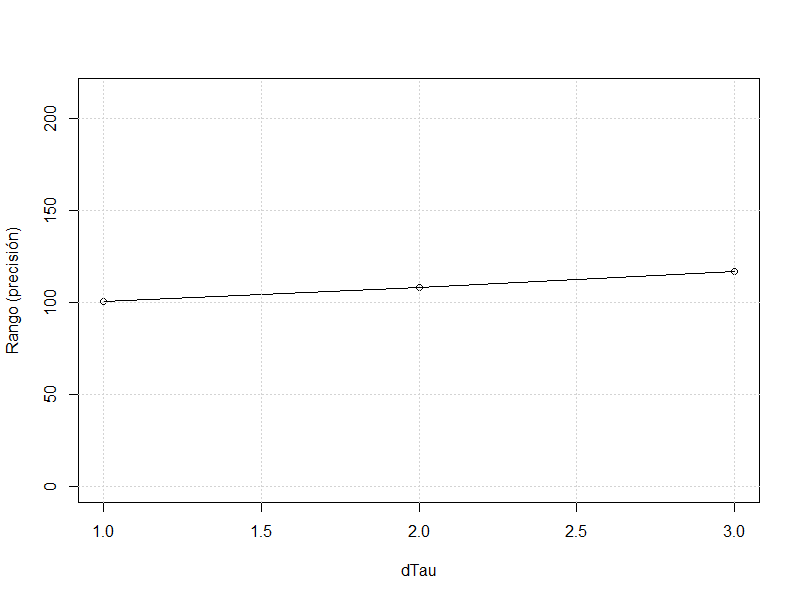
\includegraphics[width=0.75\textwidth]{images/p/p-MEdTau.png}
    }
    \subfigure[Clasificador]{
    
        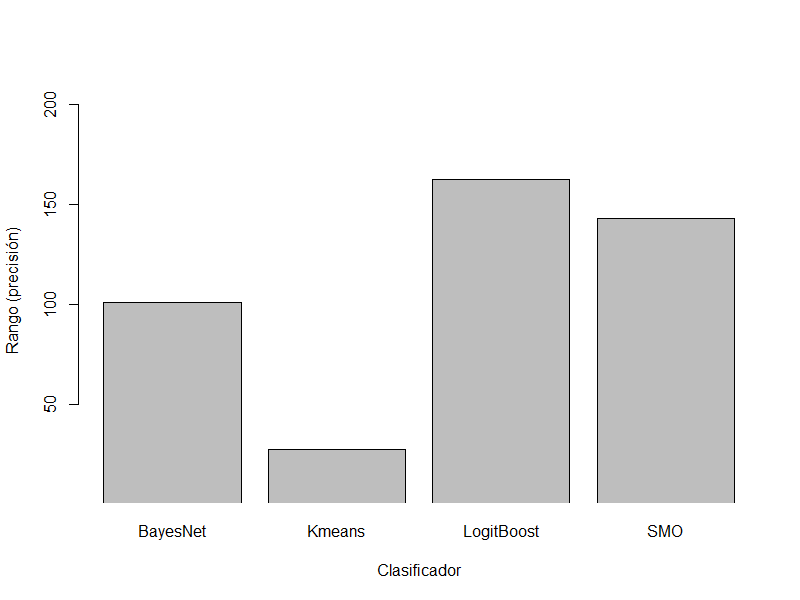
\includegraphics[width=0.75\textwidth]{images/p/p-MEclasificador.png}
    }
\caption{Promedio del efecto de los factores $\Delta \tau$ y clasificador sobre la precisión.}
\label{tab:ME-B}
\end{figure}


La interacción de segundo nivel entre $\Delta \tau$ y el clasificador se puede apreciar en la figura \ref{tab:2I-B}. 
Aquí se puede notar claramente el gran peso que tiene el clasificador sobre la precisión, donde se pueden notar dos picos muy marcados, uno bajo en Kmeans y uno alto en LogitBoost. 
La diferencia entre cada uno de los clasificadores en términos de $\Delta \tau$ no es muy fuerte, especialmente con Kmeans. Se da un comportamiento interesante, en todos los clasificadores menos en Kmeans, donde la diferencia entre los promedios varía mucho con respecto a $\Delta \tau$.

\begin{figure}[H]

    \centering
	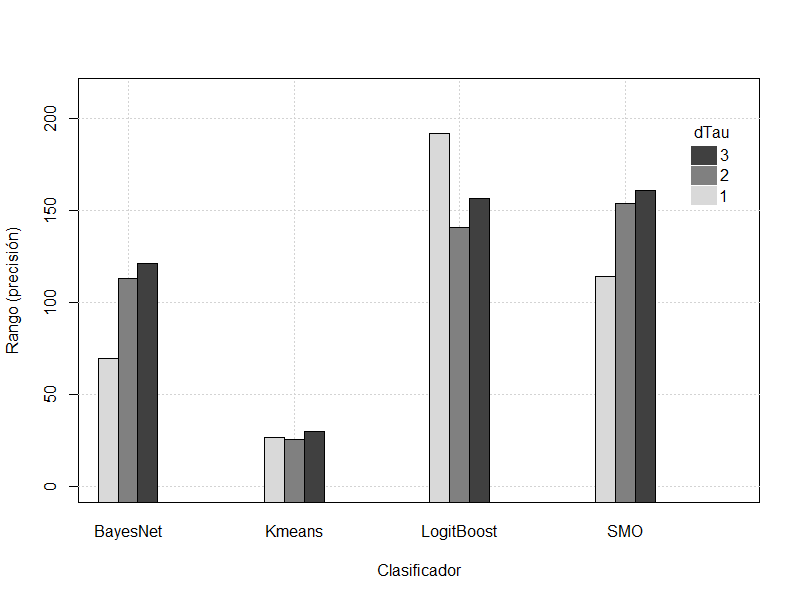
\includegraphics[width=0.75\textwidth]{images/p/p-2I.png}
\caption{Promedio de la interacción de segundo nivel entre $\Delta \tau$ y el clasificador para la precisión en el experimento B.}
\label{tab:2I-B}
\end{figure}

La figura \ref{fig:pix-p} grafica los clasificadores contra la cantidad de píxeles en promedio usados en cada configuración de parámetros de frecuencia.
La cantidad promedio de píxeles utilizada se calcula con la siguiente fórmula:

\begin{equation}
%(360/phi)*(len/rho)	((trazMax+trazMin)/2)*numTraz/tau
    \text{promedio píxeles} = \frac{trazMax + trazMin}{2} * \frac{numTraz}{\Delta \tau}
\end{equation}

Donde:
\begin{itemize}
    \item $trazMax$ es el trazo más largo que se puede hacer sobre la imagen, en este caso 500.
    \item $trazMin$ es el trazo más corto que se puede hacer sobre la imagen, en este caso 1.
    \item $numTraz$ es la cantidad de trazos que se hacen sobre la imagen según $\Delta \rho$ y $\Delta \phi$ y se calcula como se muestra a continuación:

    \begin{equation}
    %(360/phi)*(len/rho)	((trazMax+trazMin)/2)*numTraz/tau
        \text{numTraz} = \frac{360}{\Delta \phi} * \frac{trazMax}{\Delta \rho}
    \end{equation}
\end{itemize}


\begin{figure}[H]
    \centering
    	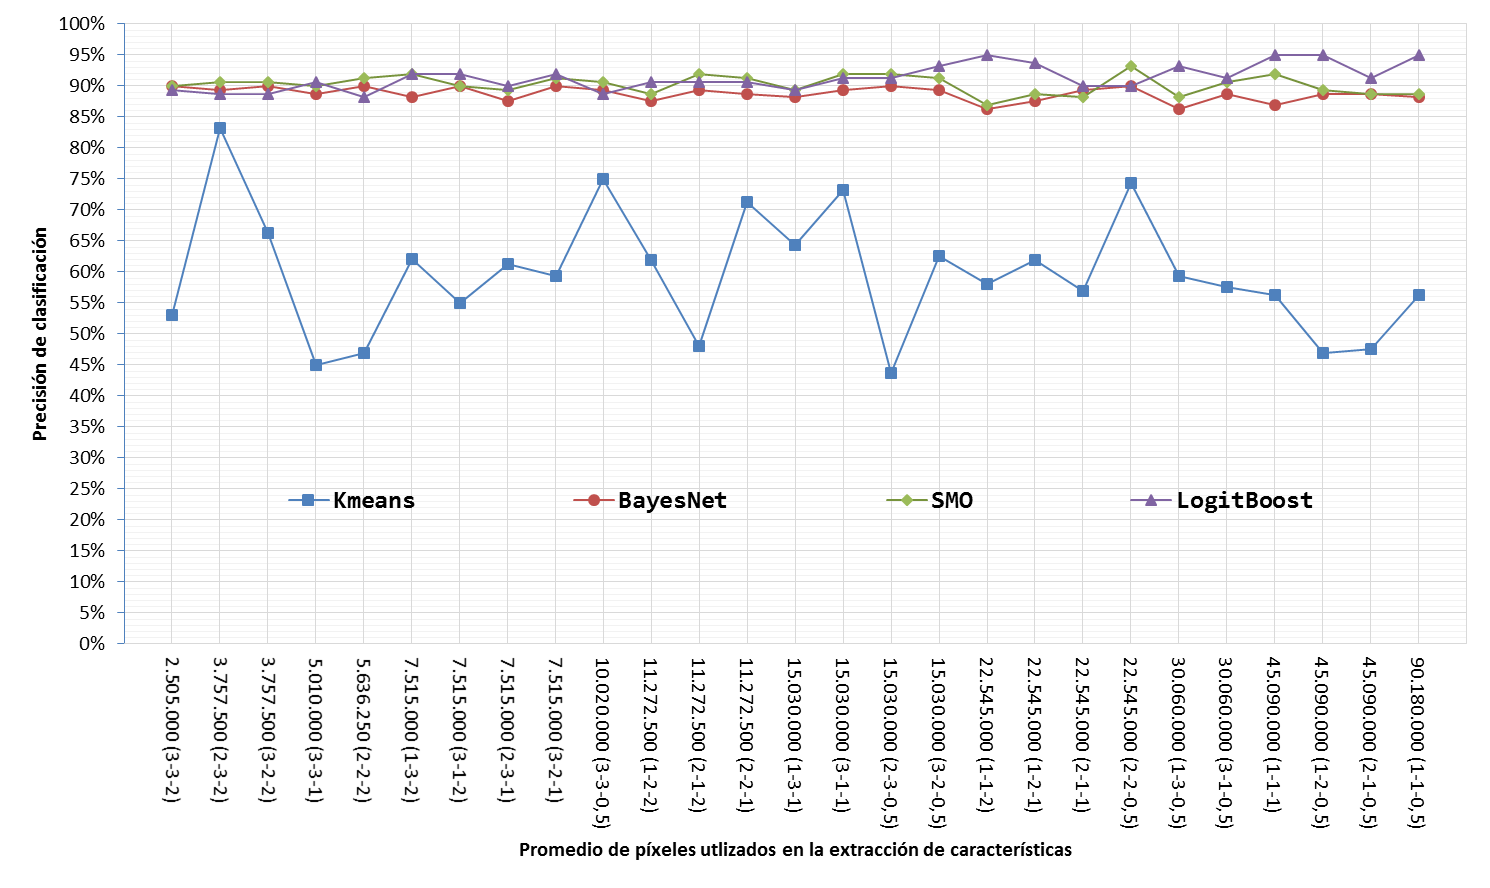
\includegraphics[width=1\textwidth]{images/p/pix-p.png}
\caption{Promedio del efecto de los factores $\Delta \tau$ y clasificador sobre la precisión.}
\label{fig:pix-p}
\end{figure}

En dicha figura se puede notar que, independientemente de la cantidad de píxeles utilizados para la extracción (por ende los parámetros de frecuencia), los clasificadores se comportan de manera similar y con poca variabilidad, con la excepción de Kmeans. LogitBoost oscila entre 0,88125 y 0,95, BayesNet entre 0,8625 y 0,9 y SMO entre 0,86875 y 0,93125.
